\documentclass[12pt,letterpaper]{article}
\usepackage{pdfpages}
\usepackage{fancyhdr}
\usepackage[colorlinks=true, urlcolor=blue, linkcolor=blue]{hyperref}
\usepackage{graphicx}
\usepackage[top=1.4in, left=0.5in, right=0.5in, bottom=0.8in]{geometry}
\usepackage[T1]{fontenc}
\usepackage{helvet}
\pagestyle{fancy}
\renewcommand{\headrulewidth}{0pt}
\renewcommand{\footrulewidth}{0pt}
\setlength{\parindent}{0em}
\setlength{\parskip}{1em}


\fancyfoot[C]{\setlength{\unitlength}{1in}\begin{picture}(5,0)\put(-1.8,-1){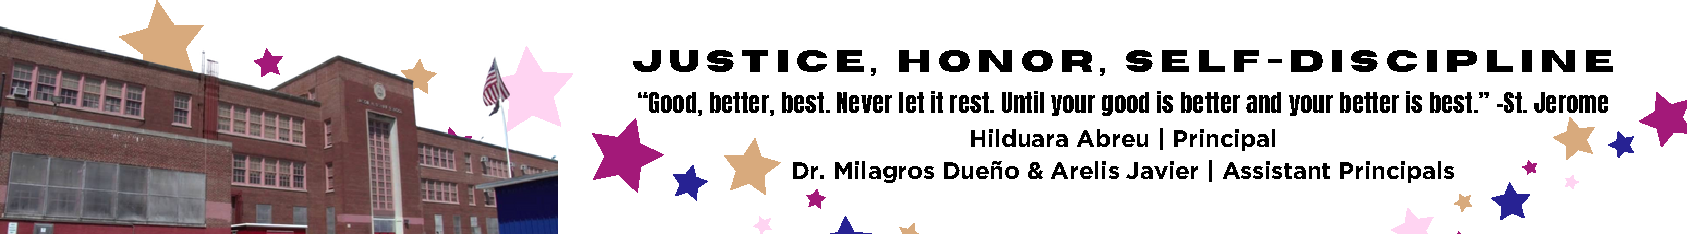
\includegraphics[width=8.8in,height=1.3in]{logo-1}}\end{picture}}
\fancyhead[C]{\setlength{\unitlength}{1in}\begin{picture}(5,0)\put(-1.9,-1){
\includegraphics[width=8.9in,height=1.3in]{logo-2}}\end{picture}}

\pagenumbering{gobble}
\addtolength{\evensidemargin}{-2in}
\addtolength{\topmargin}{-0.5in}
\addtolength{\textwidth}{0in}
%%%%%%%%%%%%%%%%%%%%%%%%%%%%%%%%%%%%%%%%%%%%%%%%%%%%%%%%%%%%%%%%%%

\begin{document}
\vspace*{0.5in}
Date: \href{https://www.ps192.org/apps/bbmessages/show_bbm.jsp?REC_ID=139439}{September 14, 2023} 

\textbf{Sujeto: Reglamento Escolar Sobre El Uso de Dispositivos Electrónicos:}

\textbf{Uso de Dispositivos Electrónicos:}

Aunque no se recomienda, los estudiantes pueden traer los siguientes artículos electrónicos a 
la escuela: teléfonos celulares; y/o sistemas portátiles de música y entretenimiento, como 
iPods y reproductores de MP3. El estudiante y/o padre es responsable de la seguridad y 
protección del dispositivo y debe saber que las instalaciones no están disponibles para cargar
dichos dispositivos en la escuela.

\textbf{Uso permitido de dispositivos electrónicos:}

Se pueden usar teléfonos celulares, dispositivos informáticos y sistemas portátiles de música y entretenimiento: Antes de las 8:00 a. m. o después de las 3:35 p. m., o en cualquier lugar
del edificio donde no sirva como distracción para las actividades educativas, incluidos 
equipos, u otros programas aprobados por la escuela.

\textbf{Uso prohibido de dispositivos electrónicos:}

Los teléfonos celulares, los dispositivos informáticos y los sistemas portátiles de música y entretenimiento no pueden:
\begin{itemize}
\item Ser encendido o utilizado durante el tiempo de instrucción, excepto para fines educativos y de instrucción con la aprobación explícita del maestro; y/o 
\item Ser encendido o utilizado durante la administración de cualquier cuestionario, prueba o examen escolar, excepto cuando dicho uso haya sido autorizado explícitamente por la escuela o esté contenido en un Programa de Educación Individualizado o Plan de Adaptación de la Sección 504; y/o
\item Estar en posesión de los estudiantes (incluso en su persona o en una bolsa) durante el horario de campana de la escuela; y/o 
\item Estar encendido o utilizado durante simulacros de incendio en la escuela u otros ejercicios de preparación para emergencias; y/o
\item Ser utilizado en baños; y/o
\item Ser usado durante el almuerzo en la cafetería y/o en el patio de la escuela; y/o
\item Úsese entre clases cuando esté en los pasillos y escaleras; y/o
\pagebreak
\vspace*{2cm} 
\item Ser utilizado en violación de cualquier disposición del Código de Disciplina del DOE, la política de la escuela, la Disposición A-413 del Canciller y/o la Política de Seguridad y Uso Aceptable de Internet del DOE ("IAUSP").
\end{itemize}
\textbf{Violaciones por el uso de Dispositivos Electrónicos:}

Las violaciones de esta política estarán sujetas a medidas disciplinarias, que pueden incluir:
\begin{itemize}
\item Confiscación del dispositivo: los artículos confiscados solo se devolverán al padre/tutor legal después de una conferencia de comportamiento sobre la violación del código de disciplina escolar; y/o
\item Revocación de privilegios: los estudiantes pueden perder el privilegio de traer artículos electrónicos a la escuela; y/o
\item Medida disciplinaria adicional: siguiendo las intervenciones de orientación y las respuestas disciplinarias descritas en el Código disciplinario del DOE.
\end{itemize}

En unidad,


\includegraphics[width=0.2\textwidth]{hil_signature}

\textbf{Principal}

\textit{La Escuela donde El Aprendisaje es Divertido!}

\url{www.ps192.org}

\end{document}
